% Signpost with loads applied
% Author: Paul Gessler
\documentclass{article}
\usepackage{tikz}             % TikZ and PGF
% Vector Styles
\tikzstyle{load}   = [ultra thick,-latex]
\tikzstyle{stress} = [-latex]
\tikzstyle{dim}    = [latex-latex]
\tikzstyle{axis}   = [-latex,black!55]

% Drawing Views
\tikzstyle{isometric}=[x={(0.710cm,-0.410cm)},y={(0cm,0.820cm)},z={(-0.710cm,-0.410cm)}]
\tikzstyle{dimetric} =[x={(0.935cm,-0.118cm)},y={(0cm,0.943cm)},z={(-0.354cm,-0.312cm)}]
\tikzstyle{dimetric2}=[x={(0.935cm,-0.118cm)},z={(0cm,0.943cm)},y={(+0.354cm,+0.312cm)}]
\tikzstyle{trimetric}=[x={(0.926cm,-0.207cm)},y={(0cm,0.837cm)},z={(-0.378cm,-0.507cm)}]

\begin{document}
\begin{center}
  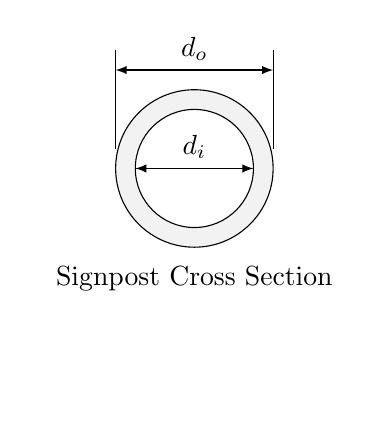
\begin{tikzpicture}
    \node (origin) at (0,0) {}; % shift relative baseline
    \coordinate (O) at (2,3);
    \draw[fill=gray!10] (O) circle (1);
    \draw[fill=white] (O) circle (0.75) node[below,yshift=-1.125cm] {Signpost Cross Section};
    \draw[dim] (O) ++(-0.75,0) -- ++(1.5,0) node[midway,above] {$d_i$};
    \draw[dim] (O) ++(-1,1.25) -- ++(2,0) node[midway,above] {$d_o$}; 
    \foreach \x in {-1,1} {
      \draw (O) ++(\x,0.25) -- ++(0,1.25);
    }
  \end{tikzpicture}%
  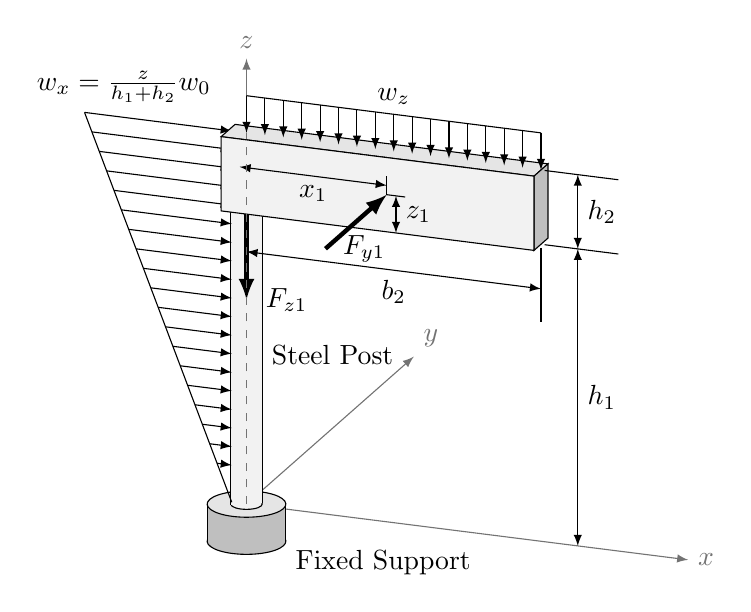
\begin{tikzpicture}[dimetric2]
        \coordinate (O) at (0,0,0);
        \draw[axis] (O) -- ++(6,0,0) node[right] {$x$};
        \draw[axis] (O) -- ++(0,6,0) node[above right] {$y$};
        \draw[axis] (O) -- ++(0,0,6) node[above] {$z$};
        \draw[fill=gray!50] (0,0,-0.5) circle (0.5); 
        \fill[fill=gray!50] (-0.46,-0.2,-0.5) -- (0.46,0.2,-0.5) -- (0.46,0.2,0) -- (-0.46,-0.2,0) -- cycle;
        \draw[fill=gray!20] (O) circle (0.5);
    \draw (0.46,0.2,-0.5) -- ++(0,0,0.5) node[below right,pos=0.0] {Fixed Support};
    \draw (-0.46,-0.2,-0.5) -- ++(0,0,0.5);
    \draw[fill=gray!10] (O) circle (0.2);
    \fill[fill=gray!10] (-0.175,-0.1,0) -- (0.175,0.1,0) -- ++(0,0,4) -- (-0.175,-0.1,4) -- cycle;
    \draw (-0.175,-0.1,0) -- ++(0,0,4);
    \draw (0.175,0.1,0) -- ++(0,0,4) node[right,midway] {Steel Post};
    \draw (4,0,3.95) -- ++(0,0,-1);
    \foreach \z in {0.5,0.75,...,5} {
      \draw[-latex] (-2*\z/5-0.2,0,\z) -- (-0.2,0,\z);
    }
    \draw[load] (0,0,4) -- ++(0,0,-1.25) node[right,xshift=0.1cm] {$F_{z1}$};
    \draw[fill=gray!20] (-0.25,-0.25,5) -- (4,-0.25,5) -- (4,+0.25,5) -- (-0.25,+0.25,5) -- cycle; 
    \draw[fill=gray!50] (+4.00,-0.25,4) -- (4,+0.25,4) -- (4,+0.25,5) -- (+4.00,-0.25,5) -- cycle; 
    \draw[fill=gray!10] (-0.25,-0.25,4) -- (4,-0.25,4) -- (4,-0.25,5) -- (-0.25,-0.25,5) -- cycle; 
    \draw (4.05,0,4) -- ++(1,0,0);
    \draw (4.05,0,5) -- ++(1,0,0);
    \draw[dim] (4.5,0,0) -- ++(0,0,4) node[midway,right] {$h_1$};
    \draw[dim] (4.5,0,4) -- ++(0,0,1) node[midway,right] {$h_2$};
    \draw[dim] (0,0,3.4) -- ++(4,0,0) node[midway,below] {$b_2$};
    \coordinate (P) at (2,-0.25,4.5);
    \draw (P) -- ++(0,0,0.25);
    \draw (P) -- ++(0.25,0,0);
    \draw[dim] (2.125,-0.25,4.5) -- ++(0,0,-0.5) node[midway,right] {$z_1$};
    \draw[dim] (2,-0.25,4.625) -- ++(-2,0,0) node[midway,below] {$x_1$};
    \draw[load] (2,-2.45,4.5) -- ++(0,2.2,0) node[pos=0.0,right,xshift=0.08cm] {$F_{y1}$};
    \draw[axis,dashed,-] (O) -- (0,0,5);
    \draw (0,0,5.5) -- ++(4,0,0) node[midway,above] {$w_{z}$};
    \foreach \x in {0,0.25,...,4} {
      \draw[-latex] (\x,0,5.5) -- ++(0,0,-0.5);
    }
    \draw (-0.2,0,0) -- ++(-2,0,5) node[above,xshift=0.5cm] {$w_{x}=\frac{z}{h_1+h_2} w_0$};
  \end{tikzpicture} %
\end{center}
\end{document}